
\documentclass{IFFranciscoME}\usepackage[]{graphicx}\usepackage[]{color}
%% maxwidth is the original width if it is less than linewidth
%% otherwise use linewidth (to make sure the graphics do not exceed the margin)
\makeatletter
\def\maxwidth{ %
  \ifdim\Gin@nat@width>\linewidth
    \linewidth
  \else
    \Gin@nat@width
  \fi
}
\makeatother

\definecolor{fgcolor}{rgb}{0.345, 0.345, 0.345}
\newcommand{\hlnum}[1]{\textcolor[rgb]{0.686,0.059,0.569}{#1}}%
\newcommand{\hlstr}[1]{\textcolor[rgb]{0.192,0.494,0.8}{#1}}%
\newcommand{\hlcom}[1]{\textcolor[rgb]{0.678,0.584,0.686}{\textit{#1}}}%
\newcommand{\hlopt}[1]{\textcolor[rgb]{0,0,0}{#1}}%
\newcommand{\hlstd}[1]{\textcolor[rgb]{0.345,0.345,0.345}{#1}}%
\newcommand{\hlkwa}[1]{\textcolor[rgb]{0.161,0.373,0.58}{\textbf{#1}}}%
\newcommand{\hlkwb}[1]{\textcolor[rgb]{0.69,0.353,0.396}{#1}}%
\newcommand{\hlkwc}[1]{\textcolor[rgb]{0.333,0.667,0.333}{#1}}%
\newcommand{\hlkwd}[1]{\textcolor[rgb]{0.737,0.353,0.396}{\textbf{#1}}}%

\usepackage{framed}
\makeatletter
\newenvironment{kframe}{%
 \def\at@end@of@kframe{}%
 \ifinner\ifhmode%
  \def\at@end@of@kframe{\end{minipage}}%
  \begin{minipage}{\columnwidth}%
 \fi\fi%
 \def\FrameCommand##1{\hskip\@totalleftmargin \hskip-\fboxsep
 \colorbox{shadecolor}{##1}\hskip-\fboxsep
     % There is no \\@totalrightmargin, so:
     \hskip-\linewidth \hskip-\@totalleftmargin \hskip\columnwidth}%
 \MakeFramed {\advance\hsize-\width
   \@totalleftmargin\z@ \linewidth\hsize
   \@setminipage}}%
 {\par\unskip\endMakeFramed%
 \at@end@of@kframe}
\makeatother

\definecolor{shadecolor}{rgb}{.97, .97, .97}
\definecolor{messagecolor}{rgb}{0, 0, 0}
\definecolor{warningcolor}{rgb}{1, 0, 1}
\definecolor{errorcolor}{rgb}{1, 0, 0}
\newenvironment{knitrout}{}{} % an empty environment to be redefined in TeX

\usepackage{alltt}
\usepackage{tikz}
\usetikzlibrary{mindmap,shadows}
\usepackage[spanish,es-nodecimaldot]{babel}
\usepackage{ragged2e}
\usepackage{etoolbox}
\usepackage{subcaption}

% Information boxes
\newcommand*{\info}[4][16.3]{%
  \node [ annotation, #3, scale=0.85, text width = #1em,
          inner sep = 2mm ] at (#2) {%
  \list{$\bullet$}{\topsep=0pt\itemsep=0pt\parsep=0pt
    \parskip=0pt\labelwidth=8pt\leftmargin=8pt
    \itemindent=0pt\labelsep=2pt}%
    #4
  \endlist
  };
}

\title[Open Data Day]{ConoceR para CompartiR}
\subtitle{Fuentes de Informaci\'on Abierta y Visualizaciones con R.}

\author{%
    \textbf{Francisco Mu\~noz Elguez\'abal} \\
    Ingenier\'ia Financiera - ITESO\\
    \textcolor{blue}{\texttt{if.francisco.me@gmail.com}}}

\institute[ITESO]
{  }

\date{5.Marzo.2016}



\IfFileExists{upquote.sty}{\usepackage{upquote}}{}
\begin{document}

% -- ----------------------------------------------------------------------------- -- %
% -- Portada ---------------------------------------------------------- Lamina (1) -- %
% -- ----------------------------------------------------------------------------- -- %

\begin{frame}{}
  \titlepage
\end{frame}

% -- ----------------------------------------------------------------------------- -- %
% -- ----------------------------------------------------- Proyecto PAP Lamina (2) -- %
% -- ----------------------------------------------------------------------------- -- %

\begin{frame}{Mapa de contenidos}

\begin{figure}[H]
\centering
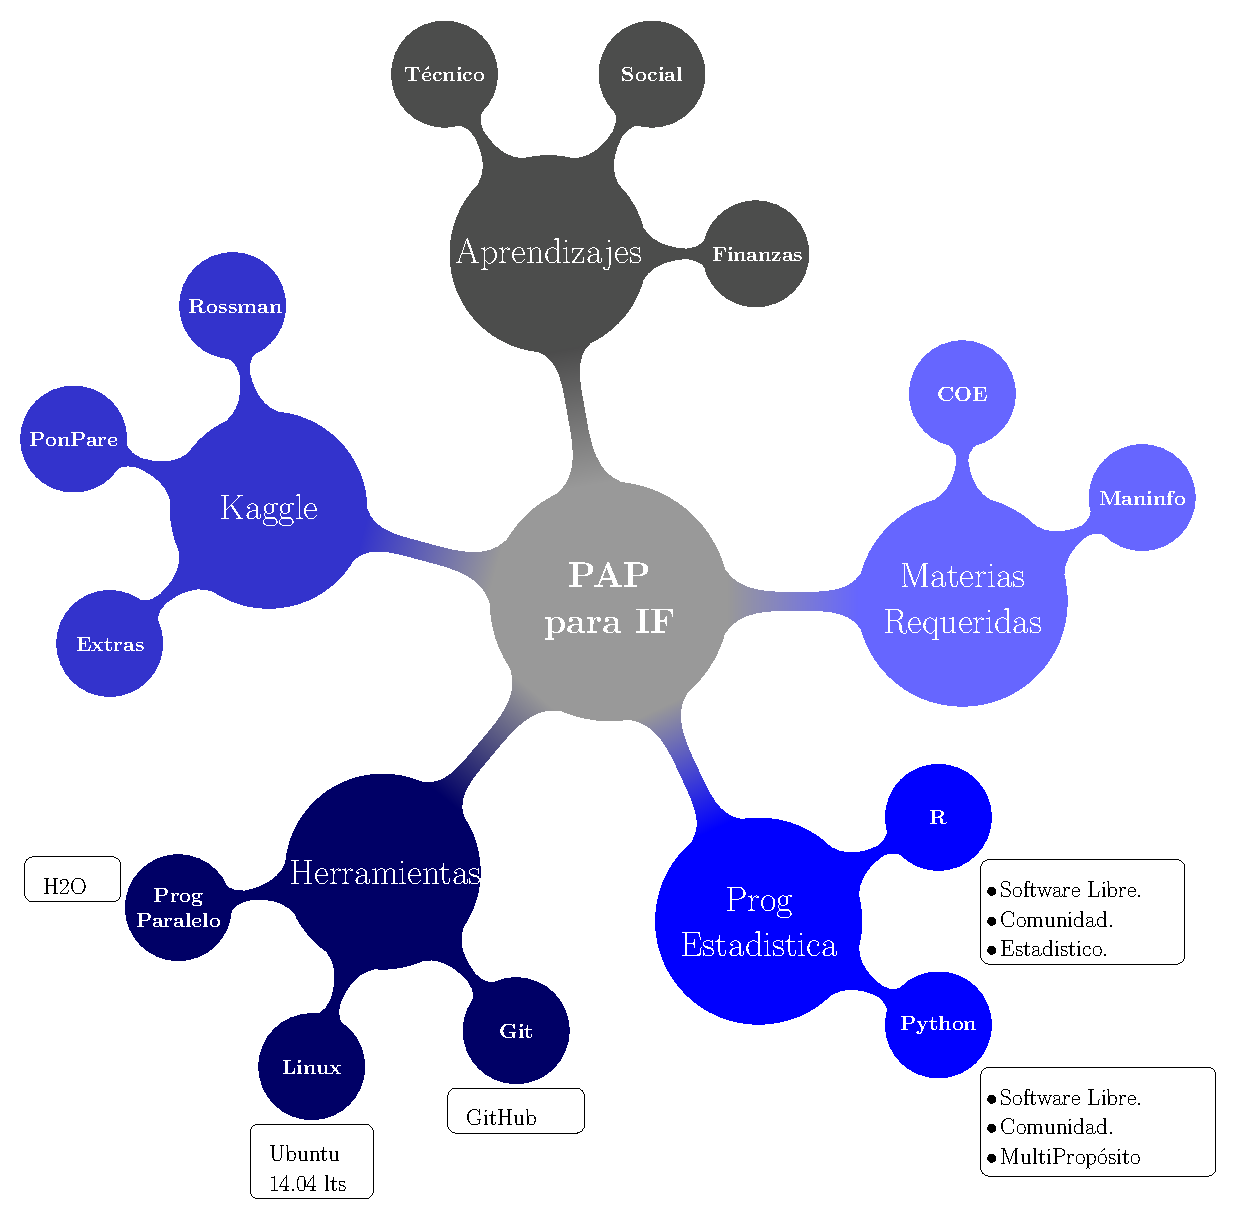
\includegraphics[scale=.36]{MindMap.pdf}
\end{figure}

\end{frame}

% -- ----------------------------------------------------------------------------- -- %
% -- Historia --------------------------------------------------------- Lamina (1) -- %
% -- ----------------------------------------------------------------------------- -- %

\begin{frame}{Definici\'on y Versiones}

\begin{block}{Definici\'on de CRAN}
\textit{R is a language and environment for \textbf{statistical computing and graphics}. 
R was created by \textbf{R}oss Ihaka and \textbf{R}obert Gentleman at the University of
Auckland, New Zealand. It is a \textbf{GNU project} which is similar to \textbf{S language}
and environment which was developed at \textbf{Bell Laboratories} (formerly AT\&T, 
now Lucent Technologies) by John Chambers and colleagues.}
\end{block}

\begin{block}{Actualmente}

\begin{itemize}
  \item MultiPlataforma: \textbf{Windows, MacOS, Linux}
  \item Editor: \textbf{RStudio 0.99.891}
  \item \'Ultima Versi\'on: \textbf{3.2.4}
  \item Paquetes existentes: \textbf{8041}
\end{itemize}

\end{block}

\end{frame}

% -- ----------------------------------------------------------------------------- -- %
% -- Historia --------------------------------------------------------- Lamina (1) -- %
% -- ----------------------------------------------------------------------------- -- %

\begin{frame}{Fuentes de Informaci\'on y Recursos}

\begin{itemize}

  \item C.R.A.N (\textbf{C}omprehensive \textbf{R} \textbf{A}rchive \textbf{N}etwork) \\
  \textcolor{blue}{ \href{https://cran.r-project.org}
  {www.cran.r-project.org}}
  
  \item M.R.A.N (\textbf{M}icrosoft \textbf{R} \textbf{A}pplication \textbf{N}etwork) \\
  \textcolor{blue}{\href{https://mran.revolutionanalytics.com}
  {www.mran.revolutionanalytics.com}}
  
  \item RBloggers: Blog de Blogs \\
  \textcolor{blue}{\href{http://www.r-bloggers.com/}
  {www.r-bloggers.com/}}

  \item RDocumentation: Documentaci\'on y busqueda de funciones \\
  \textcolor{blue}{\href{www.rdocumentation.com}{www.rdocumentation.com}}
  
  \item RStudio: Info y \textit{Cheatsheets} del Editor \\
  \textcolor{blue}{\href{https://www.rstudio.com/resources/cheatsheets/}
  {www.rstudio.com/resources/cheatsheets/}}
  
  \item RPubs: Publicaci\'on de documentos con Texto + C\'odigo \\
  \textcolor{blue}{\href{www.rpubs.com}
  {www.rpubs.com}}
  
  \item IDRE: \textbf{I}nstitute for \textbf{D}igital \textbf{R}esearch and 
  \textbf{E}ducation \textit{UCLA} \\ 
  \textcolor{blue}{\href{http://www.ats.ucla.edu/stat/r}
  {www.ats.ucla.edu/stat/r}}
  
\end{itemize}

\end{frame}

% -- ----------------------------------------------------------------------------- -- %
% -- Historia --------------------------------------------------------- Lamina (1) -- %
% -- ----------------------------------------------------------------------------- -- %

\begin{frame}{¿ Quien utiliza R ?}


Todos estos

\end{frame}

% -- ----------------------------------------------------------------------------- -- %
% -- -------------------------- Herramientas Computacionales Utilizadas Lamina (6) -- %
% -- ----------------------------------------------------------------------------- -- %

\begin{frame}{GITHUB para control de versiones}

\begin{figure}
\centering
\begin{subfigure}{.5\textwidth}
  \centering
  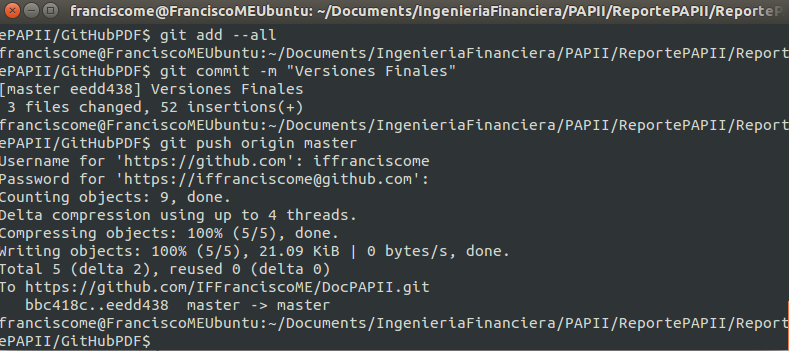
\includegraphics[width=1.1\linewidth]{figure/GitHubLINUX.png}
  \caption{GitHub en Terminal}
\end{subfigure}%
\begin{subfigure}{.5\textwidth}
  \centering
  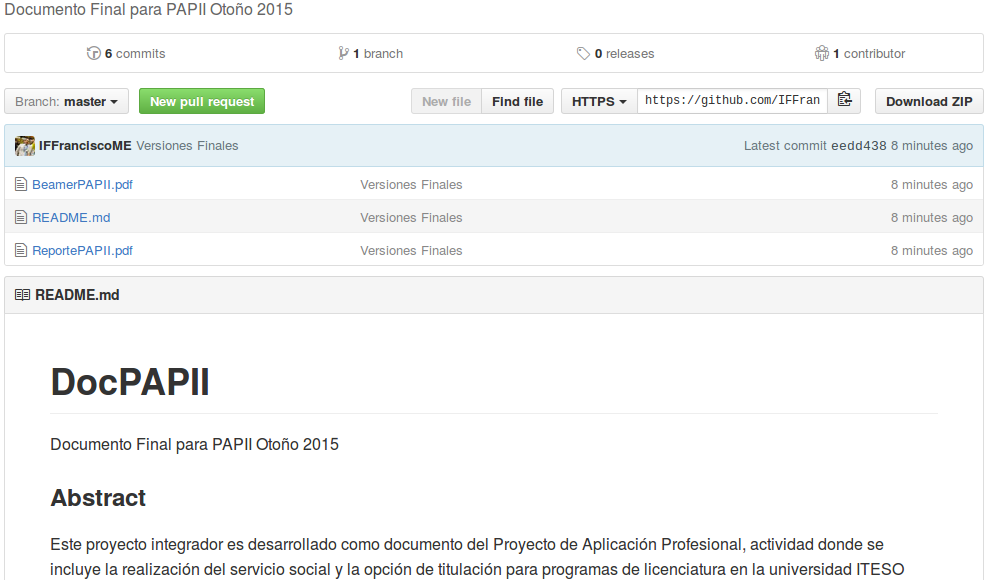
\includegraphics[width=.85\linewidth]{figure/GitHubWEB.png}
  \caption{GitHub en WEB}
\end{subfigure}
\end{figure}

\begin{figure}[H]
\centering
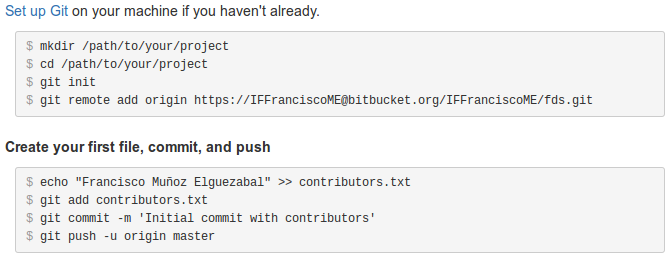
\includegraphics[scale=.34]{figure/SetupGit.png}
\end{figure}

\end{frame}

% -- ----------------------------------------------------------------------------- -- %
% -- -------------------------- Herramientas Computacionales Utilizadas Lamina (6) -- %
% -- ----------------------------------------------------------------------------- -- %

\begin{frame}{Aplicaciones de muestra}

Miner\'ia de texto b\'asica con TwitteR
Visualizaci\'on b\'asica de Imp\'acto econ\'omico de tipo de cambio

\end{frame}

% -- ----------------------------------------------------------------------------- -- %
% -- -------------------------- Herramientas Computacionales Utilizadas Lamina (6) -- %
% -- ----------------------------------------------------------------------------- -- %

\begin{frame}{Visualizando TwitteR I}

\end{frame}

% -- ----------------------------------------------------------------------------- -- %
% -- -------------------------- Herramientas Computacionales Utilizadas Lamina (6) -- %
% -- ----------------------------------------------------------------------------- -- %

\begin{frame}{Visualizando TwitteR II}

\end{frame}

% -- ----------------------------------------------------------------------------- -- %
% -- -------------------------- Herramientas Computacionales Utilizadas Lamina (6) -- %
% -- ----------------------------------------------------------------------------- -- %

\begin{frame}{Visualizando TwitteR III}

\end{frame}

% -- ----------------------------------------------------------------------------- -- %
% -- -------------------------- Herramientas Computacionales Utilizadas Lamina (6) -- %
% -- ----------------------------------------------------------------------------- -- %

\begin{frame}{Visualizando Tipo de Cambio I}

\end{frame}

% -- ----------------------------------------------------------------------------- -- %
% -- -------------------------- Herramientas Computacionales Utilizadas Lamina (6) -- %
% -- ----------------------------------------------------------------------------- -- %

\begin{frame}{Visualizando Tipo de Cambio II}

\end{frame}

% -- ----------------------------------------------------------------------------- -- %
% -- -------------------------- Herramientas Computacionales Utilizadas Lamina (6) -- %
% -- ----------------------------------------------------------------------------- -- %

\begin{frame}{Visualizando Tipo de Cambio III}





\end{frame}

\end{document}
